\documentclass[12pt]{article} % "article" is one of the standard LaTeX styles
% note that other styles are available and anything appropriate is acceptable.
% All journals have their own style files defining the look of the article.
% For these reports it's best to stick to one-column formatting.

%%%%%%%%%%%%%%%%%
\iffalse
\usepackage{graphicx} % for including graphics
\usepackage{amsmath} % useful maths macros, including \text
\usepackage[a4paper, total={6in, 9.5in}]{geometry} % set the paper/text sizes
\fi
%%%%%%%%%%%%%%%%%%%%

%\usepackage{apacite}
%\usepackage[round]{natbib}
%\usepackage[colorlinks=true,linkcolor=blue]{hyperref}
\usepackage[a4paper, total={6in, 9.5in}]{geometry} % set the paper/text sizes

\usepackage{amsmath}
\usepackage{graphicx}
\usepackage[english]{babel}
\usepackage[absolute,overlay]{textpos}
\usepackage{caption}
%\captionsetup{labelformat=empty,labelsep=none}
%\captionsetup{format=hang}
%\captionsetup{font=scriptsize}
\usepackage{amssymb}
\usepackage{tcolorbox}
\usepackage{tipa}
\usepackage{siunitx}
\usepackage{adjustbox}
\usepackage{setspace}
\usepackage{lipsum}
\usepackage{physics}
\usepackage{hyperref}
\usepackage{flowchart}
\usetikzlibrary{arrows}
\usepackage{booktabs}
\usepackage{longtable}
\usepackage{layout}
\usepackage{geometry}
%\geometry{left=12mm}


\hypersetup{colorlinks,
citecolor=blue,linkcolor=red, urlcolor=blue
}
\usepackage{qrcode}
\renewcommand{\vec}[1]{\boldsymbol{#1}}
\newcommand{\Hmns}{\tiny\textrm{H}}
\usepackage{media9}
\usepackage{aasmacros}
\usepackage{multimedia}
\usepackage{sidecap}
\usepackage{pdfpages}
\usepackage{xspace}
\usepackage{float}
%\usepackage{minted}
\usepackage{indentfirst}
\usepackage[round]{natbib}

%\usepackage[breaklinks,colorlinks,
   %urlcolor=blue,citecolor=blue,linkcolor=blue]{hyperref}
   

\newcommand{\bilby}{{\sc Bilby}\xspace}
\newcommand{\PyCBC}{{\sc PyCBC}\xspace}
\newcommand{\IPython}{{\sc IPython}\xspace}
\newcommand{\Python}{{\sc Python}\xspace}
\newcommand{\Numpy}{{\sc NumPy}\xspace}
\newcommand{\astropy}{{\sc Astropy}\xspace}
\newcommand{\R}{{\sc R}\xspace}


\newcommand{\be}{\begin{equation}}
\newcommand{\ee}{\end{equation}}
\newcommand{\ba}{\begin{eqnarray}}
\newcommand{\ea}{\end{eqnarray}}
\newcommand{\nn}{\nonumber}

\renewcommand{\arraystretch}{1.5}


\usepackage{etoolbox}

\makeatletter

% Patch case where name and year are separated by aysep
\patchcmd{\NAT@citex}
  {\@citea\NAT@hyper@{%
     \NAT@nmfmt{\NAT@nm}%
     \hyper@natlinkbreak{\NAT@aysep\NAT@spacechar}{\@citeb\@extra@b@citeb}%
     \NAT@date}}
  {\@citea\NAT@nmfmt{\NAT@nm}%
   \NAT@aysep\NAT@spacechar\NAT@hyper@{\NAT@date}}{}{}

% Patch case where name and year are separated by opening bracket
\patchcmd{\NAT@citex}
  {\@citea\NAT@hyper@{%
     \NAT@nmfmt{\NAT@nm}%
     \hyper@natlinkbreak{\NAT@spacechar\NAT@@open\if*#1*\else#1\NAT@spacechar\fi}%
       {\@citeb\@extra@b@citeb}%
     \NAT@date}}
  {\@citea\NAT@nmfmt{\NAT@nm}%
   \NAT@spacechar\NAT@@open\if*#1*\else#1\NAT@spacechar\fi\NAT@hyper@{\NAT@date}}
  {}{}

\makeatother


\usepackage{fancyhdr}
\fancypagestyle{CVfooter}
{
 \lhead{Gerald Leung}
 \chead{SPD Checks}
 \rhead{\today}
 \lfoot{\small{}}
 \cfoot{\small{}}
 \rfoot{\small{\thepage}}
 %\renewcommand{\headrulewidth}{0.5pt}
 %\renewcommand{\footrulewidth}{0.5pt}
}



\begin{document}
\title{Notes on Scottish Postcode Directory Quality Checking}
\author{Gerald Leung\\Public Health Scotland}
\date{Draft version: \today}
\maketitle
\tableofcontents
\section{Introduction}
\pagestyle{CVfooter}

In this short document, we summarise the process of
the Scottish Postcode Directory (SPD) file checks from the
National Records of Scotland (NRS) by the Geospatial Team at
Public Health Scotland (PHS). In short, NRS updates
SPD files twice a year, around March and September\footnote{\url{https://www.nrscotland.gov.uk/statistics-and-data/geography/nrs-postcode-extract}}. The Geospatial Team
will then conduct quality checks of the updated files
and compare any changes with the previous version.
They will then produce lookup files in various
formats, such as \texttt{.csv}. This
document focuses on summarising the processes of quality
checking (QC)
and lookup files production using \R.
Here we also reproduce a brief summary
of the data, which can be found in Appendix \ref{appendix:dict}.
Full details can be found through the \href{https://www.nrscotland.gov.uk/files//statistics/geography/2021-2/spd-datadictionary-2021-2.pdf}{data dictionary} provided by the NRS,
or accessed through
\begin{verbatim}
//PHIBCS/PHI/Referencing & Standards/GPD/1_Geography
/Scottish Postcode Directory/Source Data/2021_2
/ISD Data Dictionary_2021-2
\end{verbatim}
for the \textbf{2021-2} version.

\section{Initial Quality Checks}
The \R scripts are located in 
\begin{verbatim}
//PHIBCS/PHI/Referencing & Standards/GPD/5_GitHub/GPD/Geography
/Scottish Postcode Directory
\end{verbatim}
and the Standard Operating Procedures (SOPs) are located in
\begin{verbatim}
//PHIBCS/PHI/Referencing & Standards/GPD/1_Geography
/Scottish Postcode Directory/SOPs.
\end{verbatim}
The source files can be found in
\begin{verbatim}
//PHIBCS/PHI/Referencing & Standards/GPD/1_Geography
/Scottish Postcode Directory/Source Data.
\end{verbatim}
They can be accessed through the organisation's VPN.
The first QC is done through the \R script \texttt{1\_Check NRS SPD.R}.

In short, this script conducts a general initial
QC of the newest version of SPD files and compares
changes with the previous version. Figure \ref{fig:block1}
shows roughly the structure of the script and the QC process.

To start with, all empty rows contained in the files
are removed and the files are combined. The user will then
record the total number of records and postcode types.
Sanity checks are conducted to make sure there are
no blank entries for Health Board and Council Areas etc.
Checks are then carried out to make sure columns are
aligned correctly. For example, between Health Board Area
Code and Council Area Code columns. This is generally done
by assigning a number to the case when a particular
column does not have an expected code that should match
with the other column. 
During 2019, eight postcodes moved from Glasgow City Council to
North Lanarkshire Council. Extensive checks are then carried
out to make sure there are no blank fields. Checks are also
carried out to make sure there are no English voting codes included.
Finally, the script makes sure that mappings are done correctly,
such as Data Zones and Health Boards.

The script also makes comparisons with previous SPD files.
For instance,it checks for changes in postcodes
(some have been deleted), different data zones and
health boards etc.

\begin{figure}[h!]
%\centering
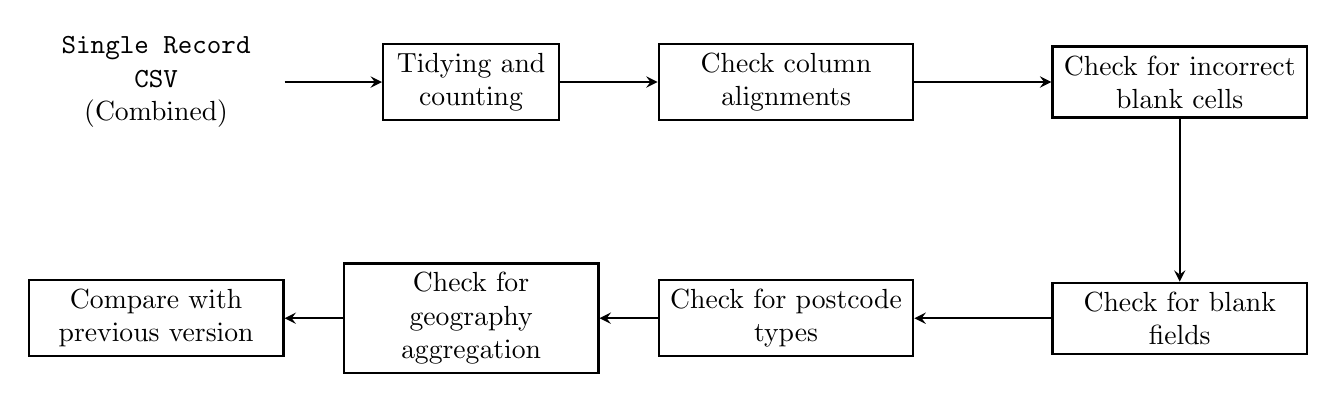
\begin{tikzpicture}[>=stealth, thick]

\node (P) at (-17,8) [text width=3cm, minimum height=0.8cm, align=flush center] 
{\texttt{Single Record CSV}\\(Combined)};

\node (A) at (-13,8) [draw, process, text width=2cm, minimum height=0.8cm, align=flush center] 
{Tidying and counting};

\node (B) at (-9,8)  [draw, process, text width=3cm, minimum height=0.8cm, align=flush center] 
{Check column alignments};

%\node (B1) at (-4,9.5)  [draw, process, text width=3cm, minimum height=0.8cm, align=flush center] 
%{\texttt{OUTCAR}};

\node (B2) at (-4,8)  [draw, process, text width=3cm, minimum height=0.8cm, align=flush center] 
{Check for incorrect blank cells};

\node (B3) at (-4,5)  [draw, process, text width=3cm, minimum height=0.8cm, align=flush center] 
{Check for blank fields};

\node (B4) at (-9,5)  [draw, process, text width=3cm, minimum height=0.8cm, align=flush center] 
{Check for postcode types};

\node (B5) at (-13,5)  [draw, process, text width=3cm, minimum height=0.8cm, align=flush center] 
{Check for geography aggregation};

\node (B6) at (-17,5)  [draw, process, text width=3cm, minimum height=0.8cm, align=flush center] 
{Compare with previous version};

%\node (B3) at (-4,6.5)  [draw, process, text width=3cm, minimum height=0.8cm, align=flush center] 
%{\texttt{ORBCAR}};

%\draw[->] (A) to node[midway,above=0.3em,align=center]{test} (B);
%\draw[<-] (A)  --node[midway,above=0.3,align=center,text width=4cm]{Input parameters} [midway,below=0.3,align=center,text width=4cm]{Manual input} +(-180:4cm) ;
%\draw[<-] (A)  --node[above]{Input parameters} +(-180:4cm);
\draw[->] (P) -- (A);

\draw[->] (A) -- (B);
%\draw[->] (B) -- (B1);
\draw[->] (B) -- (B2);
%\draw[->] (B) -- (B3);
\draw[->] (B2) -- (B3);
\draw[->] (B3) -- (B4);
\draw[->] (B4) -- (B5);
\draw[->] (B5) -- (B6);


\end{tikzpicture}
\caption{Schematic diagram of the initial QC process.}\label{fig:block1}
\end{figure}
 
\section{Lookup Files}
The next step of the process is to produce lookup files for
other uses and analysis within the organisation.




\iffalse
\begin{figure}[h!]
\centering
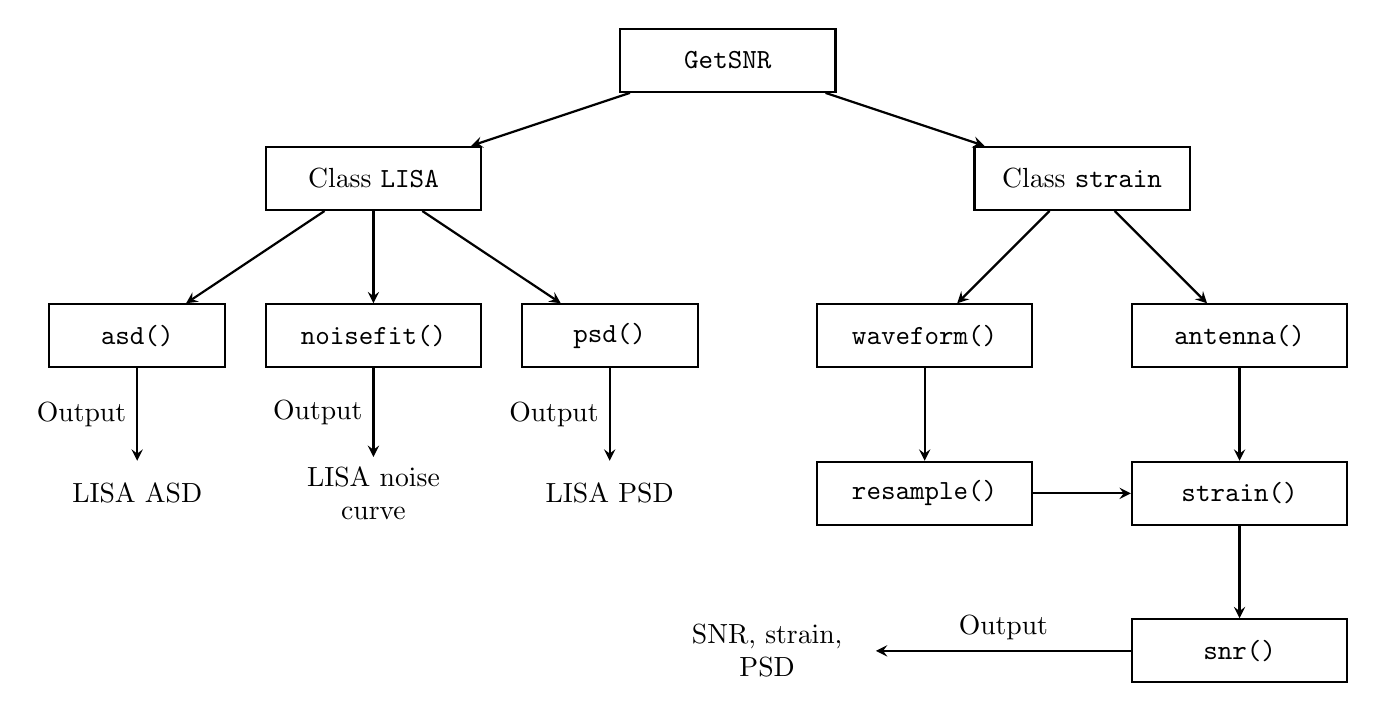
\begin{tikzpicture}[>=stealth, thick]

\node (A) at (-3.5,0) [draw, process,text width=2.5cm, minimum height=0.8cm, align=flush center] 
{\texttt{GetSNR}};

\node (B1) at (-8,-1.5) [draw, process,text width=2.5cm, minimum height=0.8cm, align=flush center] 
{Class \texttt{LISA}};

\node (C1) at (-11,-3.5) [draw, process,text width=2cm, minimum height=0.8cm, align=flush center] 
{\texttt{asd()}};

\node (C2) at (-8,-3.5) [draw, process,text width=2.5cm, minimum height=0.8cm, align=flush center] 
{\texttt{noisefit()}};

\node (C3) at (-5,-3.5) [draw, process,text width=2cm, minimum height=0.8cm, align=flush center] 
{\texttt{psd()}};


\node (B2) at (1,-1.5) [draw, process,text width=2.5cm, minimum height=0.8cm, align=flush center] 
{Class \texttt{strain}};

\node (D1) at (-1,-3.5) [draw, process,text width=2.5cm, minimum height=0.8cm, align=flush center] 
{\texttt{waveform()}};

\node (D2) at (-1,-5.5) [draw, process,text width=2.5cm, minimum height=0.8cm, align=flush center] 
{\texttt{resample()}};

\node (D3) at (3,-3.5) [draw, process,text width=2.5cm, minimum height=0.8cm, align=flush center] 
{\texttt{antenna()}};

\node (D4) at (3,-5.5) [draw, process,text width=2.5cm, minimum height=0.8cm, align=flush center] 
{\texttt{strain()}};

\node (D5) at (3,-7.5) [draw, process,text width=2.5cm, minimum height=0.8cm, align=flush center] 
{\texttt{snr()}};

\node (D6) at (-3,-7.5) [text width=2.5cm, minimum height=0.8cm, align=flush center] 
{SNR, strain, PSD};

\node (C4) at (-11,-5.5) [text width=2.5cm, minimum height=0.8cm, align=flush center] 
{LISA ASD};

\node (C5) at (-8,-5.5) [text width=2.5cm, minimum height=0.8cm, align=flush center] 
{LISA noise curve};

\node (C6) at (-5,-5.5) [text width=2.5cm, minimum height=0.8cm, align=flush center] 
{LISA PSD};

%\draw[->] (A) to node[midway,above=0.3em,align=center]{test} (B);
%\draw[<-] (A)  --node[midway,above=0.3,align=center,text width=4cm]{Input parameters} [midway,below=0.3,align=center,text width=4cm]{Manual input} +(-180:4cm) ;
%\draw[<-] (A)  --node[above]{Input parameters} +(-180:4cm);
\draw[->] (A) -- (B1);
\draw[->] (A) -- (B2);
\draw[->] (B1) -- (C1);
\draw[->] (B1) -- (C2);
\draw[->] (B1) -- (C3);
\draw[->] (B2) -- (D1);
\draw[->] (D1) -- (D2);
\draw[->] (B2) -- (D3);
\draw[->] (D3) -- (D4);
\draw[->] (D4) -- (D5);
\draw[->] (D2) -- (D4);
\draw[->] (D5) to node[midway,above=0.3,align=center]{Output} (D6);
\draw[->] (C1) to node[midway,left=0.3,align=center]{Output} (C4);
\draw[->] (C2) to node[midway,left=0.3,align=center]{Output} (C5);
\draw[->] (C3) to node[midway,left=0.3,align=center]{Output} (C6);

\end{tikzpicture}
\caption{Schematic diagram of the \texttt{GetSNR} pipeline. The diagram shows two classes, \texttt{LISA} and \texttt{strain}, and their respective functions and outputs.}\label{fig:block2}
\end{figure}
\fi
\newgeometry{left=10mm}

\appendix
\section{Appendix: Data Dictionary}\label{appendix:dict}

\begin{longtable}{|| m{.45\textwidth} | m{.13\textwidth} | m{.5\textwidth}||} 
\hline
\textbf{Name} & \textbf{Type} & \textbf{Notes} \\
\hline\hline
Postcode & Character & The Royal Mail postcode. Consists of area, district, sector and unit. E.g. AB1 0AA.\\ \hline
SplitChar & Character & A, B, C \\ \hline
PostcodeDistrict & Character & Postcode District. E.g. AB1. \\ \hline
PostcodeSector & Character & Postcode Sector. E.g. AB1 0.\\ \hline
DateOfIntroduction & Date & Postcode introduction date. Currently shown as $\#\#\#\#$ instead of a date. \\ \hline
DateOfDeletion & Date & Postcode deletion date.
Similarly to date of introduction. \\ \hline
PostcodeType & Character & Small (S) or Large (L).\\ \hline
LinkedSmallUserPostcode & Character & Small User postcode that
contains the grid reference of the Large User postcode.\\ \hline
LinkedSmallUserPostcodeSplitChar & Character & A, B, C\\ \hline
Imputed & Character & Whether postcode's higher area values
have been inputed.\\ \hline
DeliveryPointCount & Integer & The Royal Mail delivery point count.\\ \hline
DeliveryPointCountNonResidential & Integer & Non-residential delivery point count.\\ \hline
HouseholdCount & Integer & The Royal Mail Household count.\\ \hline
GridReferenceEasting & Character & Grid reference easting.\\ \hline
GridReferenceNorthing & Character & Grid reference northing.\\ \hline
Latitude & Numeric & Coordinates in degrees.\\ \hline
Longitude & Numeric & Coordinates in degrees.\\ \hline
SplitIndicator & Character & Split postcode indicator. Y/N.\\ \hline
CouncilArea2019Code & Character & Identifies a 2019 Council Area.\\ \hline
UKParliamentaryConstituency2005Code & Character & 2005 UK Parliamentary Constituency.\\ \hline
ScottishParliamentaryRegion2021Code & Character & 2021 Scottish Parliamentary Region.\\ \hline

\caption{Data dictionary of the SPD file. Reproduced from NRS.} % needs to go inside longtable environment
\label{tab:myfirstlongtable}
\end{longtable}
%\restoregeometry
%\end{table} 


%\bibliographystyle{ieeetr}
%\bibliographystyle{yahapj}
%\bibliography{slidescites}


\end{document}